\documentclass[10pt]{article}
\usepackage[usenames]{color} %used for font color
\usepackage{amssymb} %maths
\usepackage{amsmath} %maths
\usepackage[utf8]{inputenc} %useful to type directly diacritic characters
\usepackage{pgfplots}
\usepackage{booktabs}
\usepackage{graphicx}
\usepackage[letterpaper, portrait, margin=1.5in]{geometry}
\begin{document}
\subsection*{MSDS600 Week 4 Assignment - Nathan Worsham}
The six data sets given to analyze all have one thing in common: that the Mean and Median are very close if not the same on all distributions. If there is an exception, it would be N1 and N2 whose Mean and Median are not exactly right on top of each other but still relatively very close. For the descriptive statistics of the data sets I choose to include these:
\begin{itemize}
\item Mean, Median, and Mode to show central tendency
\item Standard Deviation to show the spread of the data
\item Minimum, Maximum, and Range to show the scope
\item 1st Quartile, 3rd Quartile, and Inner Quartile Range to show the dispersion less affected by outliers (Boslaugh, 2014)
\item Continuous or Discrete, to characterize the data set as being made up of whole numbers or mimics a continuous set
\item Number of Values to get an idea of size of the data set
\item Count of Mild and Extreme Outliers along with counts at both upper and lower ends to show if there are outliers that would skew the central tendency 
\item Graphical representations\begin{itemize}
	\item Histogram, combined when comparing
	\item Boxplot, combined when comparing
\end{itemize}
\end{itemize}
To calculate many of these values I used the built-in functions of R. The exceptions would be Mode, Range, and Outliers. For mode we were provided from the reading the equation: 
\begin{verbatim}
> mde <- density(data) #use these two commands to find the most frequent number 
> mde$x[which(mde$y == max(mde$y))]
\end{verbatim}
But I found that formula was not the best answer on discrete data sets. I found a function to calculate the top 10 values, being that the top value would be the mode worked better in these instances:
\begin{verbatim}
top10 <- function(x)
{
  counts <- table(x, useNA = "always")
  head(sort(counts, decreasing = TRUE), 10)
}
\end{verbatim}
On continuous data sets, the density option worked better because the top values would often be a cluster of values with only a couple of occurrences each. To calculate range I used \verb|max(x) - min(x)|. As for outliers, according to Boslaugh (2014) "There is no absolute agreement among statisticians about how to define outliers", however there does seem to be some guidelines that are common. One is to find "mild" outliers you multiply 1.5 times the IQR then subtract or add to the outer bounds of the IQR, and then "extreme" would be 3 instead of 1.5 (Boslaugh, 2014). To do this I created a funtion:
\begin{verbatim}
outliers <- function(x){
  lowerq = quantile(x[,1])[2]
  upperq = quantile(x[,1])[4]
  iqr <- IQR(x[,1])
  mild.lower.Thresh <- lowerq - (iqr *1.5)
  mild.upper.Thresh <- upperq + (iqr *1.5)
  extreme.lower.Thresh <- lowerq - (iqr *3)
  extreme.upper.Thresh <- upperq + (iqr *3)
  mild.lower.outliers <- x[,1][ which(x[,1] < mild.lower.Thresh) ]
  extreme.lower.outliers <- x[,1][ which(x[,1] < extreme.lower.Thresh) ]
  mild.upper.outliers <- x[,1][ which(x[,1] > mild.upper.Thresh) ]
  extreme.upper.outliers <- x[,1][ which(x[,1] > extreme.upper.Thresh) ]
  mild.upper.outliers.count <- length(mild.upper.outliers)
  mild.lower.outliers.count <- length(mild.lower.outliers)
  mild.outliers.count <- mild.upper.outliers.count + mild.lower.outliers.count
  extreme.upper.outliers.count <- length(extreme.upper.outliers)
  extreme.lower.outliers.count <- length(extreme.lower.outliers)
  extreme.outliers.count <- extreme.upper.outliers.count + extreme.lower.outliers.count 
  print(paste0("Count of Mild Outliers: ",mild.outliers.count))
  print(paste0("Count of Upper Mild Outliers: ",mild.upper.outliers.count))
  print(paste0("Count of Lower Mild Outliers: ",mild.lower.outliers.count))
  print(paste0("Count of Extreme Outliers: ",extreme.outliers.count))
  print(paste0("Count of Upper Extreme Outliers: ",extreme.upper.outliers.count))
  print(paste0("Count of Lower Extreme Outliers: ",extreme.lower.outliers.count))
}
\end{verbatim}
After creating this function I realized that I should have created a function to run against all of the data sets, rather than computing the values one at a time, which is something I will remember for next time. I also found that on the comparison data sets, showing the histograms and boxplots separately was much less effective then showing them combined.
\subsection*{Binomial.csv}
\begin{table}[h!]
  \begin{center}
    \scriptsize
    \begin{tabular}{ll}
      \toprule
      paramater & value\\
      \midrule
 	Mean & 70.17\\
	Median & 70\\
	Mode & 68\\
	Standard Deviation & 4.689325\\
	Minimum & 57\\
	Maximum & 84\\
	Range & 27\\
	1st Quartile & 67\\
	3rd Quartile & 73\\
	IQR & 6\\
	Continous or Discrete & Discrete\\
	\# of Values & 1000\\ 
	\# Count of Mild Outliers & 3\\
	\# of Upper Mild Outliers & 1\\
	\# of Lower Mild Outliers & 2\\
	\# of Extreme Outliers & 0\\
       \bottomrule
    \end{tabular}
  \end{center}
\end{table}

\par
\raisebox{-.5\height}{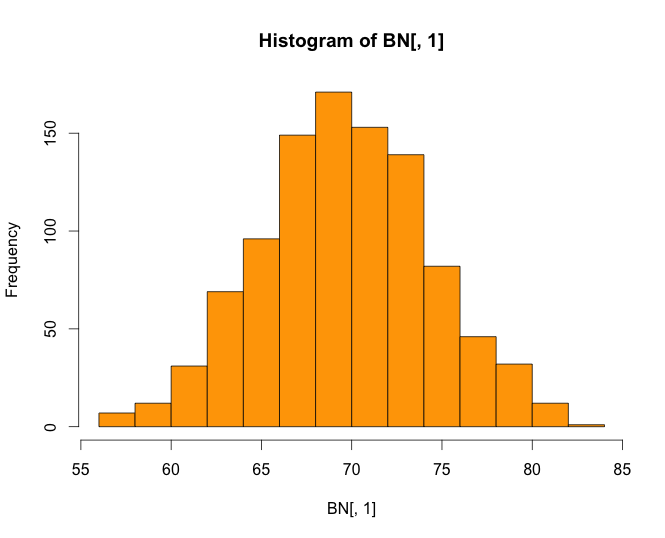
\includegraphics[width=7cm]{HistBN.png}}%
\hfill
\raisebox{-.5\height}{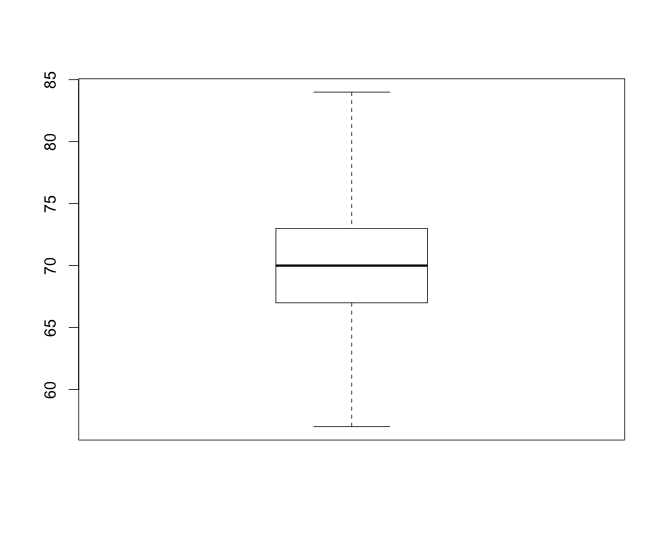
\includegraphics[width=7cm]{boxplotBN.png}}%
\par
Here we see that the Mode is below the Mean and Median. The data set close to symmetrical but skewed slightly to the left. Very little outliers, even "mild" outliers only 0.3\% of total values. \subsection*{ln.csv}
\begin{table}[h!]
  \begin{center}
    \scriptsize
    \begin{tabular}{ll}
      \toprule
      parameter & value\\
      \midrule
 	Mean & 18.99\\
	Median & 19\\
	Mode & 18\\
	Standard Deviation & 4.362612\\
	Minimum & 3\\
	Maximum & 43\\
	Range & 40\\
	1st Quartile & 16\\
	3rd Quartile & 22\\
	IQR & 6\\   
	Continous or Discrete & Discrete\\
	\# of Values & 1048576\\ 
	\# of Mild Outliers & 4750\\
	\# of Upper Mild Outliers & 4222\\
	\# of Lower Mild Outliers & 528\\
	\# of Extreme Outliers & 9\\
	\# of Upper Extreme Outliers & 9\\
	\# of Lower Extreme Outliers & 0\\
       \bottomrule
    \end{tabular}
  \end{center}
\end{table}

\par
\raisebox{-.5\height}{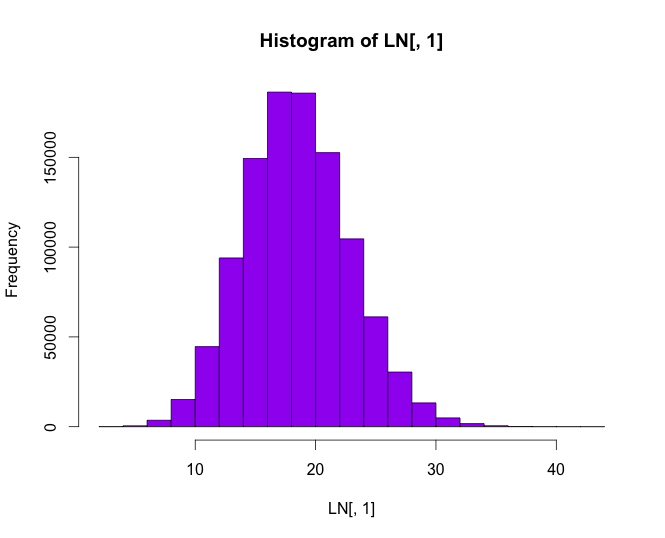
\includegraphics[width=7cm]{HistLN.png}}%
\hfill
\raisebox{-.5\height}{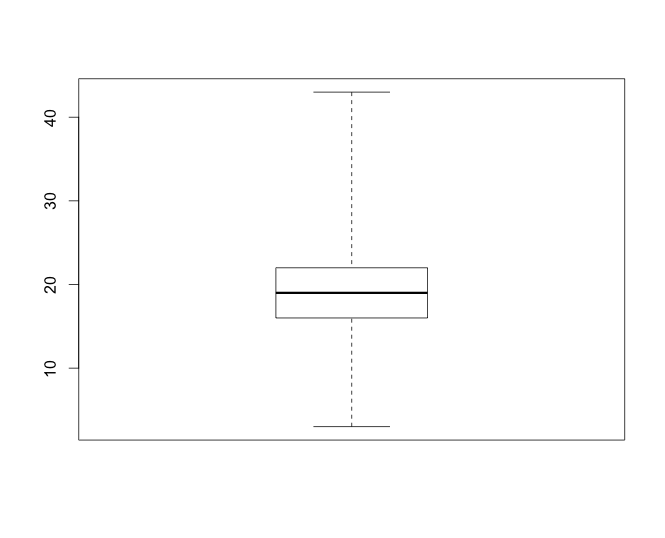
\includegraphics[width=7cm]{boxplotLN.png}}%
\par
Again the Mode is below the Median and Mean and it appears there are a lot of upper outliers, but because the total number of values is so large, the outliers only account for 0.45\% of the total. However this does help describe the right-skew which can be seen easier in the upper whisker of the boxplot.
\subsection*{BN1.csv vs BN2.csv}
\begin{table}[h!]
  \begin{center}
    \scriptsize
    \begin{tabular}{lll}
      \toprule
      parameter & BN1 & BN2\\
      \midrule
 	Mean & 9.994 & 10.997\\
	Median & 9.993 & 10.998\\
	Mode & 10.07391 & 10.94372\\
	Standard Deviation & 2.000357 & 0.9994714\\
	Minimum & 1.781 & 6.638\\
	Maximum & 18.612 & 15.161\\
	Range & 16.83086 & 8.523442\\
	1st Quartile & 8.643 & 10.321\\
	3rd Quartile & 11.343 & 11.667\\
	IQR & 2.700128 & 1.345798\\ 
	Continous or Discrete & Continuous & Continuous\\   
	\# of Values & 100000 & 100000\\  
	\# of Mild Outliers & 692 & 741\\
	\# of Upper Mild Outliers & 357 & 390\\
	\# of Lower Mild Outliers & 335 & 351\\
	\# of Extreme Outliers & 0 & 0\\
       \bottomrule
    \end{tabular}
  \end{center}
\end{table}

\par
\raisebox{-.5\height}{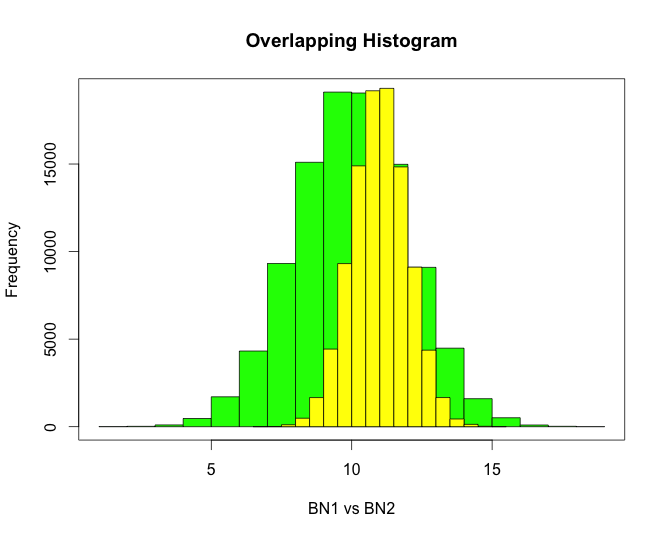
\includegraphics[width=7cm]{HistBN1vBN2.png}}%
\hfill
\raisebox{-.5\height}{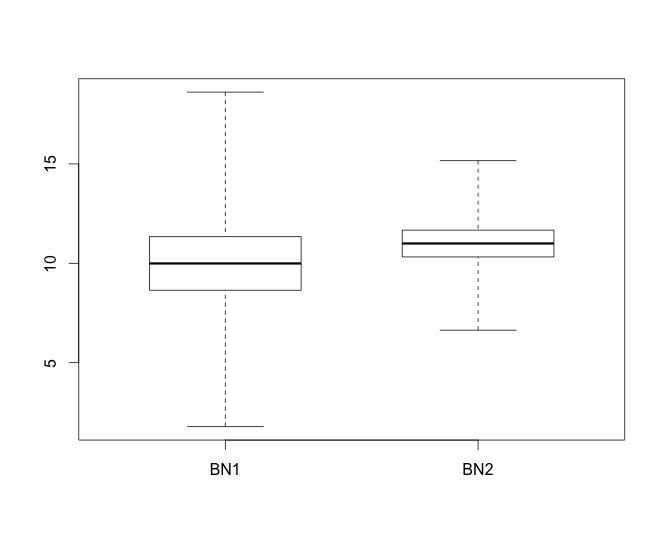
\includegraphics[width=7cm]{boxplotBN1vBN2.png}}%
\par
While BN1 and BN2 have Mean values that are close, BN1's range, IQR, and Standard Deviation are all wider (just about double) than BN2. BN2 is a much tighter distribution than BN1, this difference is clearly seen in the boxplot figure. In both data sets the Mean, Median are basically the exact same number while the Mode is extremely close. This would indicate very symmetrical distributions, which the histograms show.\\
\newline
\newline 
\newline
\newline 
\newline
\newline  
\subsection*{N1.csv vs N2.csv}

\begin{table}[h!]
  \begin{center}
    \scriptsize
    \begin{tabular}{lll}
      \toprule
      parameter & N1 & N2\\
      \midrule
 	Mean & 10.134 & 11.7082\\
	Median & 10.093 & 11.9056\\
	Mode & 9.960858 & 12.20025\\
	Standard Deviation & 1.995706 & 4.291276\\
	Minimum & 5.064 & 0.6503\\
	Maximum & 15.767 & 22.6275\\
	Range & 10.7026 & 21.97726\\
	1st Quartile & 8.774 & 9.0030\\
	3rd Quartile & 11.458 & 14.1246\\
	IQR & 2.684247 & 5.121644\\ 
	Continous or Discrete & Continuous & Continuous\\  
	\# of Values & 100 & 100\\
	\# of Mild Outliers & 1 & 2\\
	\# of Upper Mild Outliers & 1 & 1\\
	\# of Lower Mild Outliers & 0 & 1\\
	\# of Extreme Outliers & 0 & 0\\
       \bottomrule
    \end{tabular}
  \end{center}
\end{table}

\par
\raisebox{-.5\height}{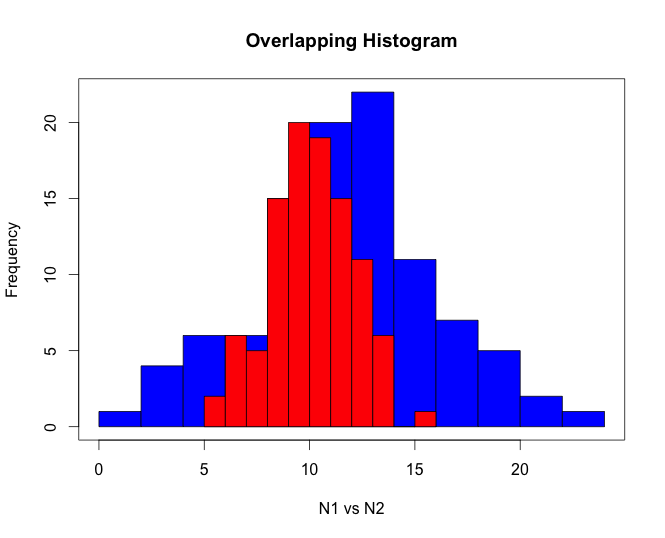
\includegraphics[width=7cm]{HistN1vN2.png}}%
\hfill
\raisebox{-.5\height}{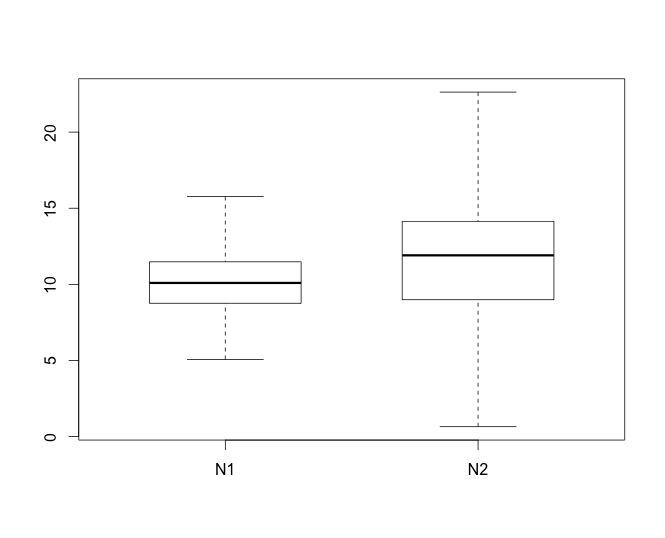
\includegraphics[width=7cm]{boxplotN1vN2.png}}%
\par
Similar to how BN1 was larger in many respects to BN2, N2 is larger than N1. It has a much wider range. N2 has several characteristics that are unusual. The Standard Deviation is comparably not that different than the Inner Quartile Range. This indicates that there is a cluster of values in the center of the distribution, but after that the values in the outer quartiles are spread apart further. The boxplot shows this well as it has long whiskers. Other notable differences is that N1's Mean is above the Median, while N2's Mean is below the Median. though the difference is minimal it would indicate the two data sets are skewed in opposite directions. 
\subsection*{Reference}
Sarah Boslaugh, 2014. Statistics in a Nutshell, 2nd Edition. Chapter 4. Descriptive Statistics and Graphic Displays.

\end{document}